\documentclass[11pt,a4paper]{article}
\usepackage[margin=2.3cm]{geometry}
\usepackage[T1]{fontenc}
\usepackage{lmodern}
\usepackage{microtype}
\usepackage{booktabs}
\usepackage{graphicx}
\usepackage{xcolor}
\usepackage{caption}
\usepackage{float}
\usepackage{enumitem}
\usepackage{amsmath}
\usepackage[hidelinks]{hyperref}
\setlist{itemsep=2pt,topsep=3pt}
\captionsetup{font=small,labelfont=bf}
\graphicspath{{figures/}}
\newcommand{\nFeatures}{31}
\newcommand{\rowsTest}{868,158}
\newcommand{\rowsTrain}{992,997}
\newcommand{\missingPct}{0.29}
\newcommand{\templateShare}{10.4}
\newcommand{\weekendRatio}{86}
\newcommand{\gapMedian}{4}
\newcommand{\gapLong}{70}
\newcommand{\nbCorr}{0.50}
\newcommand{\lgbmMAEFifteen}{48.63}
\newcommand{\lgbmWAPEFifteen}{5.31}
\newcommand{\lgbmSkillFifteen}{26.7}
\newcommand{\persMAEFifteen}{66.38}
\newcommand{\bestBaseNameFifteen}{persistence}
\newcommand{\ridgeSkillFifteen}{15.7}
\newcommand{\ridgeMAEFifteen}{55.98}
\newcommand{\lastweekMAEFifteen}{91.78}
\newcommand{\lgbmCleanMAEFifteen}{54.20}
\newcommand{\keptPct}{87.2}
\newcommand{\lgbmMAESixty}{61.15}
\newcommand{\lgbmWAPESixty}{6.67}
\newcommand{\lgbmSkillSixty}{22.0}
\newcommand{\persMAESixty}{142.01}
\newcommand{\bestBaseNameSixty}{the four-week average}
\newcommand{\ridgeSkillSixty}{4.0}
\newcommand{\ridgeMAESixty}{75.26}
\newcommand{\lastweekMAESixty}{91.74}
\newcommand{\lgbmCleanMAESixty}{67.24}
\newcommand{\ablLagsLgbm}{5.0}
\newcommand{\ablCalLgbm}{4.8}
\newcommand{\ablSeasLgbm}{2.0}
\newcommand{\ablWeatherLgbm}{-0.47}
\newcommand{\chgSteadyFifteen}{3.06}
\newcommand{\chgSuddenFifteen}{9.55}
\newcommand{\rainFifteen}{5.87}
\newcommand{\dryFifteen}{5.25}
\newcommand{\holidayFifteen}{6.04}
\newcommand{\weekdayFifteen}{5.35}
\newcommand{\lowFlowFifteen}{8.18}
\newcommand{\highFlowFifteen}{4.24}
\newcommand{\chgSteadySixty}{4.52}
\newcommand{\chgSuddenSixty}{10.36}
\newcommand{\rainSixty}{7.61}
\newcommand{\drySixty}{6.58}
\newcommand{\holidaySixty}{8.62}
\newcommand{\weekdaySixty}{6.69}
\newcommand{\lowFlowSixty}{11.17}
\newcommand{\highFlowSixty}{5.19}
\newcommand{\xgbGapFifteen}{0.11}
\newcommand{\xgbGapSixty}{0.14}
\newcommand{\ratioSixty}{0.43}
\newcommand{\mapeSixty}{14.2}
\newcommand{\mapePersSixty}{30.7}
\newcommand{\sensBest}{-1.17}
\newcommand{\nTemplateSensors}{8}
\newcommand{\templateSensorList}{2185, 2186, 2187, 2188, 2189, 2190, 2806, 2814}
\newcommand{\tplRows}{8.1}
\newcommand{\tplWapeFifteen}{1.04}
\newcommand{\otherWapeFifteen}{5.69}
\newcommand{\otherMAEFifteen}{52.04}
\newcommand{\tplWapeSixty}{1.81}
\newcommand{\otherWapeSixty}{7.11}
\newcommand{\otherMAESixty}{65.04}


\newcommand{\todo}[1]{\textcolor{red}{[#1]}}
\newcommand{\code}[1]{\texttt{#1}}

\title{\textbf{Traffic Flow Forecasting on Bay Area Freeways}\\[2pt]
\large Topic 4: Traffic Prediction -- Machine Learning Project Report}
\author{Praneeth Marudi (IMT2023555), Vinay Kusumanchi (IMT2023608),\\
Shive S Bhat (BT2024067), Mitansh (BT2024046)}
\date{\todo{course name, instructor, submission date}}

\begin{document}
\maketitle

\begin{abstract}
We forecast the traffic flow (vehicles per 15 minutes) at 100 freeway sensors in the San Francisco Bay Area, 15 and 60
minutes ahead, using the public LargeST dataset (Caltrans PeMS detectors, 2017--2019). Nine machine-learning models
(Ridge, PCA+Ridge, Decision Tree, Random Forest, AdaBoost, Gradient Boosting, XGBoost, LightGBM, CatBoost) are tuned on a
validation year, frozen, and scored once on the unseen year 2019, next to three simple baselines. All of them are checked
for leakage by tests that scramble the future. LightGBM is the most accurate model (MAE \lgbmMAEFifteen{} at 15 minutes and
\lgbmMAESixty{} at 60 minutes, i.e.\ \lgbmSkillFifteen{}\% and \lgbmSkillSixty{}\% better than the best simple baseline), although
XGBoost and CatBoost are practically tied with it. Three analyses explain the results: a feature ablation, a robustness study,
and an error analysis. A Streamlit application serves live forecasts with an uncertainty band and per-prediction
explanations. We also report where the results are less impressive than they look: eight sensors are ``template''
sensors whose data repeat last week, and a few feed outages dominate the largest errors.
\end{abstract}

\setcounter{tocdepth}{1}
\tableofcontents

% ============================================================================================================
\section{Overview and task definition}
Traffic flow changes with the hour, the weekday, holidays, weather and incidents. A forecast of the next 15 to 60 minutes
supports ramp metering, incident response and route planning, but only if it works with information that is really
available at the forecast time, and only if it also works at sensors that were not used for training.

\paragraph{Task.} At a forecast origin $t$, given everything observed \emph{before} $t$, predict the flow
$y_{t+h}$ (vehicles counted in one 15-minute bin) at one sensor, for $h=15$ and $h=60$ minutes. One model is trained per
horizon. Errors are reported in vehicles per 15 minutes (MAE, RMSE) and as WAPE, the total absolute error divided by the
total flow.

\paragraph{What was built.} (i) A cleaned dataset of 100 sensors with weather and calendar features; (ii) a fair benchmark of
3 baselines and 9 models on identical rows; (iii) three analyses (A feature ablation, D robustness, E error analysis);
(iv) a Streamlit application; (v) a Git repository with code, tests and a README that reproduces everything.

% ============================================================================================================
\section{Dataset and source}
\paragraph{Traffic.} LargeST \cite{largest} is a benchmark built from the Caltrans Performance Measurement System (PeMS)
loop detectors of California, released under CC BY-NC 4.0 and hosted on Kaggle. We use the 5-minute flow files for 2017, 2018
and 2019 and the sensor metadata (\code{ca\_meta.csv}) for District 4, the Bay Area. Flow is the number of vehicles that
passed a detector in 5 minutes, summed over the lanes.

\paragraph{Sensors.} District 4 has 2{,}352 mainline sensors. For each freeway direction we searched for 25 consecutive sensors that
lie in the five core counties, are at most 3~km apart and are at least 85\% usable in both 2017 and 2018. Four corridors were
used (Table~\ref{tab:sensors}), giving 100 sensors. In every corridor the first 20 sensors are \emph{warm} (they appear in
training) and the last 5 are \emph{cold}: they appear only in the test rows. The cold sensors measure how well a model
transfers to locations it has never been trained on.

\begin{table}[H]\centering\small
\begin{tabular}{lllccc}
\toprule
Corridor & Freeway & County & Lanes & Sensor IDs & Min. usable (\%) \\
\midrule
I580-E & I580-E & Alameda & 3--7 & 2175--2199 & 99.2 \\
US101-N & US101-N & San Mateo & 4--6 & 1416--1440 & 99.3 \\
I880-S & I880-S & Alameda & 2--6 & 2795--2819 & 99.1 \\
SR24-W & SR24-W & Alameda/Contra Costa & 3--5 & 717--741 & 99.3 \\
\bottomrule
\end{tabular}

\caption{The four corridors (25 sensors each). ``Min.\ usable'' is the lowest share of readings that are present and not a
daytime zero, over the corridor's sensors and the years 2017--2018.}\label{tab:sensors}
\end{table}

\paragraph{Weather.} Hourly precipitation, temperature and wind come from the Open-Meteo historical API (ERA5 reanalysis) \cite{openmeteo},
one point per corridor (mean coordinates of its sensors), in local time. Precipitation at hour $h$ is the sum over the hour
that ends at $h$, so the feature for an origin uses only the last completed hour. Holidays come from the Python
\code{holidays} package (US, California).

\paragraph{Reproduction.} The README explains how to download the data (\code{scripts/prepare\_data.py},
\code{scripts/fetch\_weather.py}). Selecting the sensors from the metadata and the data-quality table regenerates
\code{sensors\_100.csv} exactly.

% ============================================================================================================
\section{Exploratory data analysis}
All EDA uses 2017--2018 only; the test year is not opened. The notebook \code{01\_eda.ipynb} contains thirteen figures; the main
findings follow.

\begin{itemize}
\item \textbf{Daily and weekly rhythm.} Weekdays show commute peaks, weekends one broad midday hump, and the direction of the
corridor matters (SR-24 westbound peaks in the morning, I-580 eastbound in the evening; Figure~\ref{fig:profile}). A Sunday
carries about \weekendRatio\% of the flow of a weekday.
\item \textbf{Seasonality and weather.} Matched wet--dry comparisons (same corridor, hour, day type and month) show a small
negative rain effect on flow, about 3\% on average, so rain is a weak but real signal.
\item \textbf{Spatial dependence.} After removing each sensor's typical weekly pattern, the residuals of neighbouring sensors
correlate at about \nbCorr{} for adjacent sensors and fall with distance. This is why the sensor behind and ahead are features.
\item \textbf{Temporal dependence.} The autocorrelation peaks at 24 hours and 168 hours, which is why ``same time last week''
is a strong feature, and the error of persistence grows quickly with the horizon.
\item \textbf{Missing data.} \missingPct\% of the 15-minute values are missing after cleaning. The median gap lasts \gapMedian{} hours and \gapLong\% of the gaps are
longer than the one hour that forward-fill can bridge, so last week's value fills most of them (Figure~\ref{fig:missing}).
\end{itemize}

\begin{figure}[H]\centering
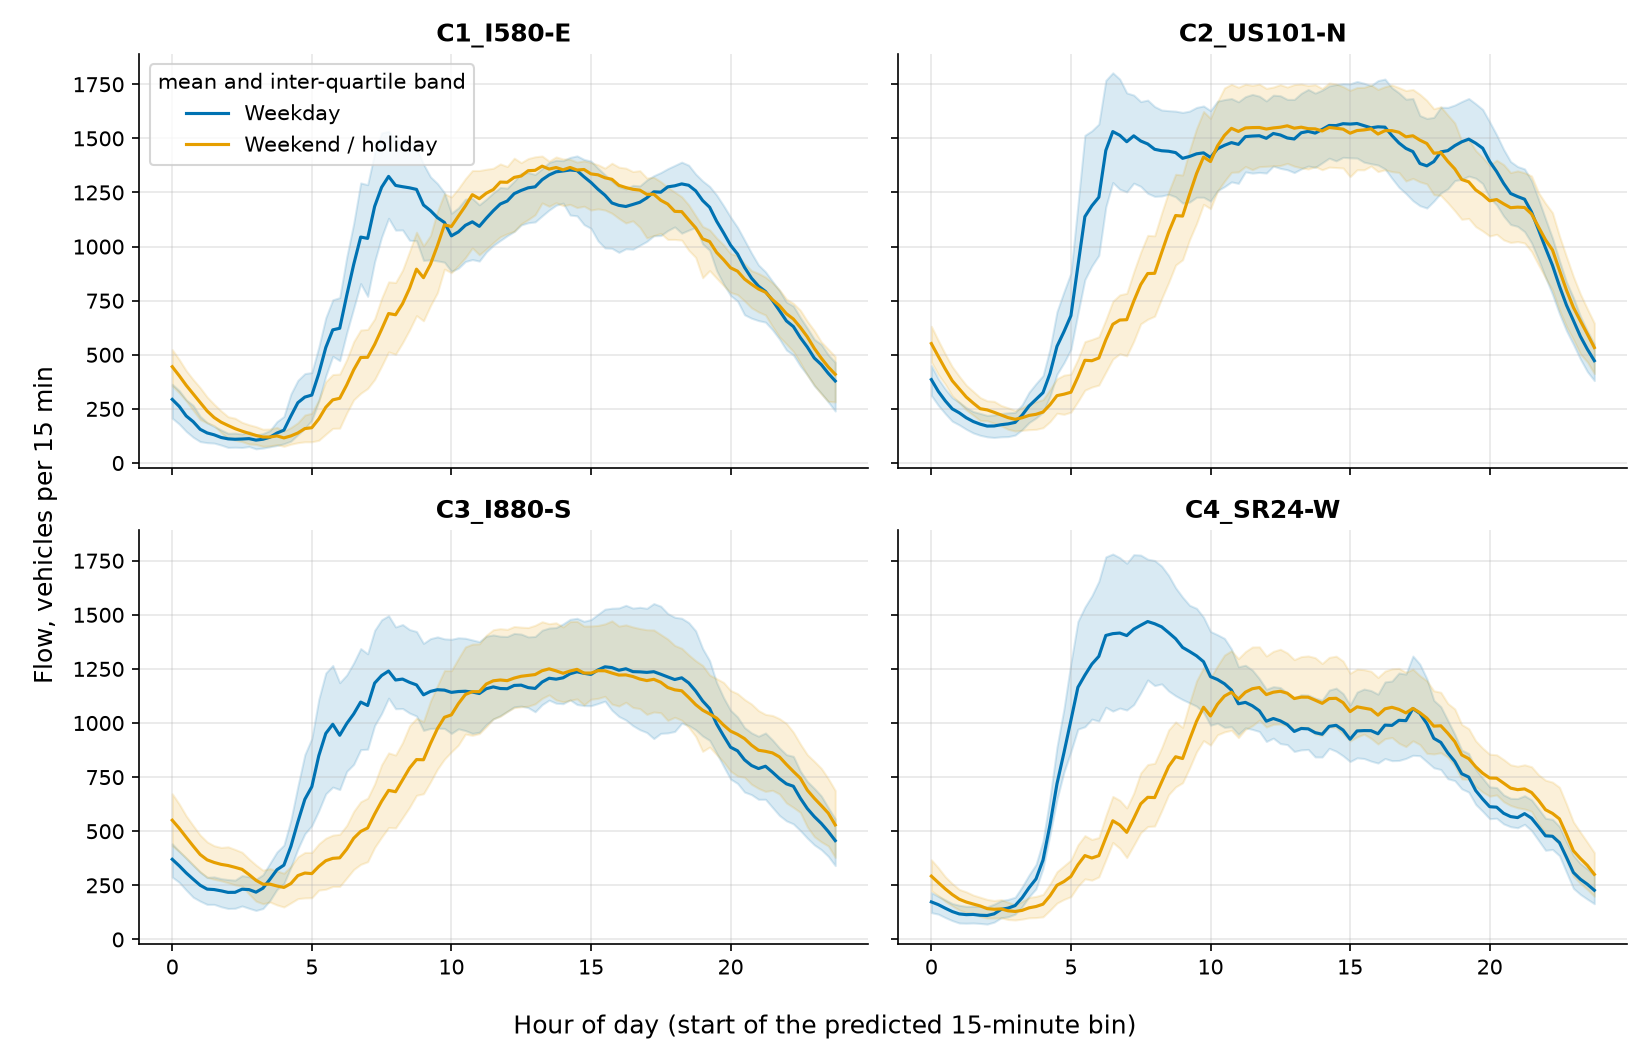
\includegraphics[width=\linewidth]{eda01_daily_profile.png}
\caption{Average daily profile of flow, weekday against weekend or holiday, per corridor.}\label{fig:profile}
\end{figure}

\begin{figure}[H]\centering
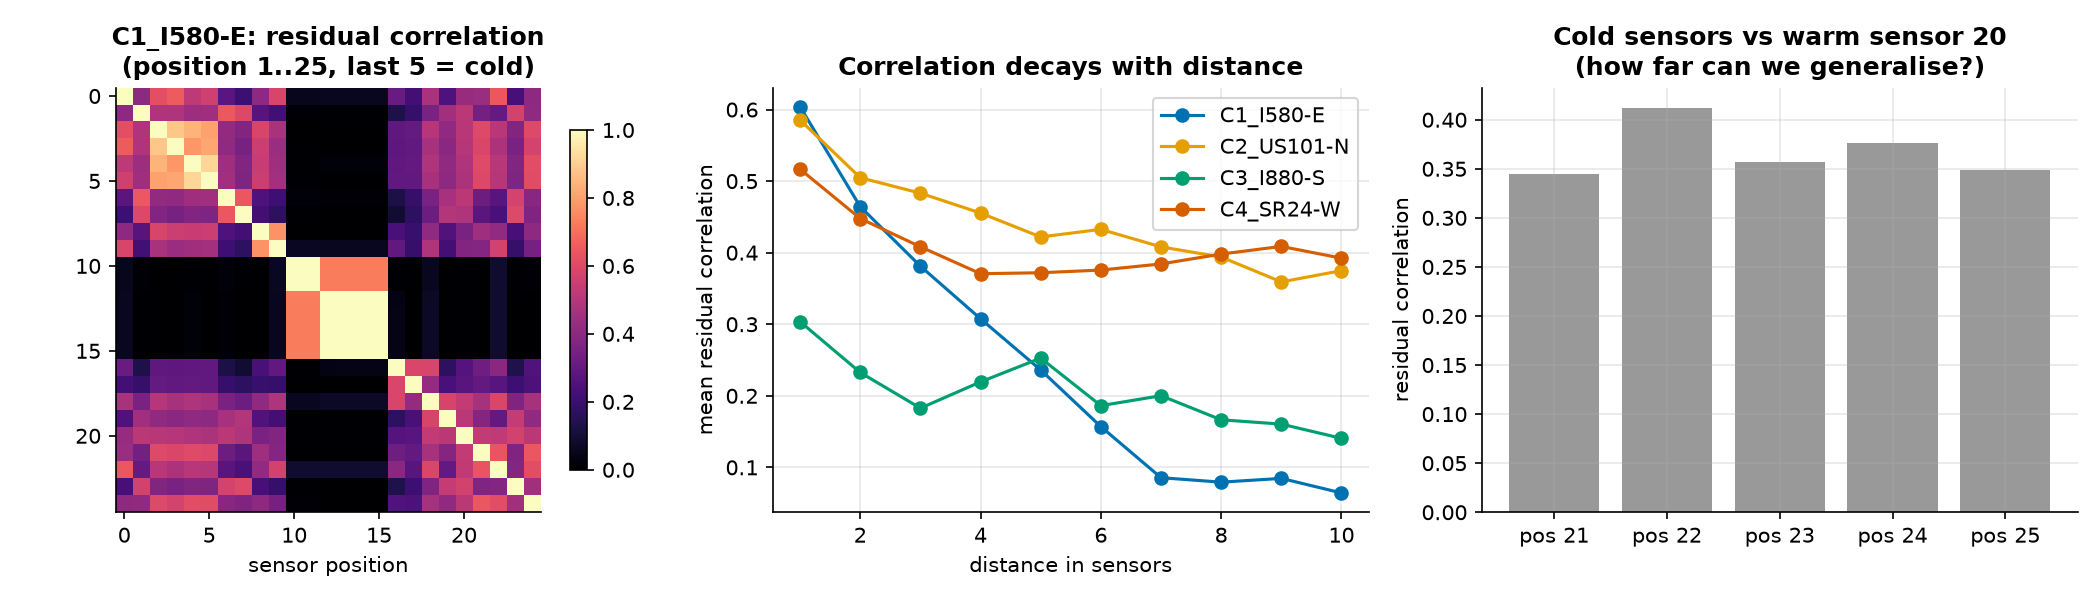
\includegraphics[width=\linewidth]{eda06_spatial_dependence.png}
\caption{Correlation of the residuals (flow minus the typical weekly pattern) between sensors, by distance along the corridor.}\label{fig:spatial}
\end{figure}

\begin{figure}[H]\centering
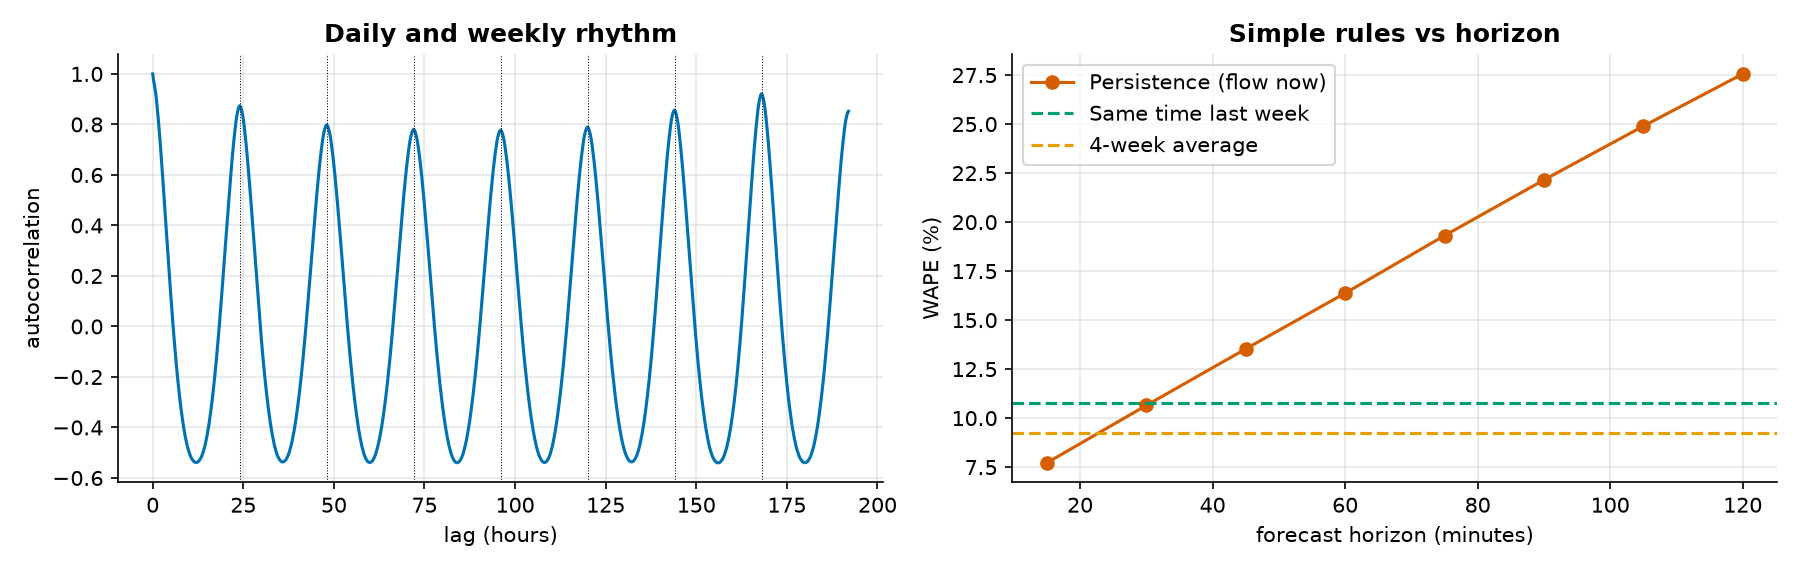
\includegraphics[width=\linewidth]{eda07_temporal_dependence.png}
\caption{Left: autocorrelation of flow. Right: error of simple rules as the forecast horizon grows.}\label{fig:temporal}
\end{figure}

\begin{figure}[H]\centering
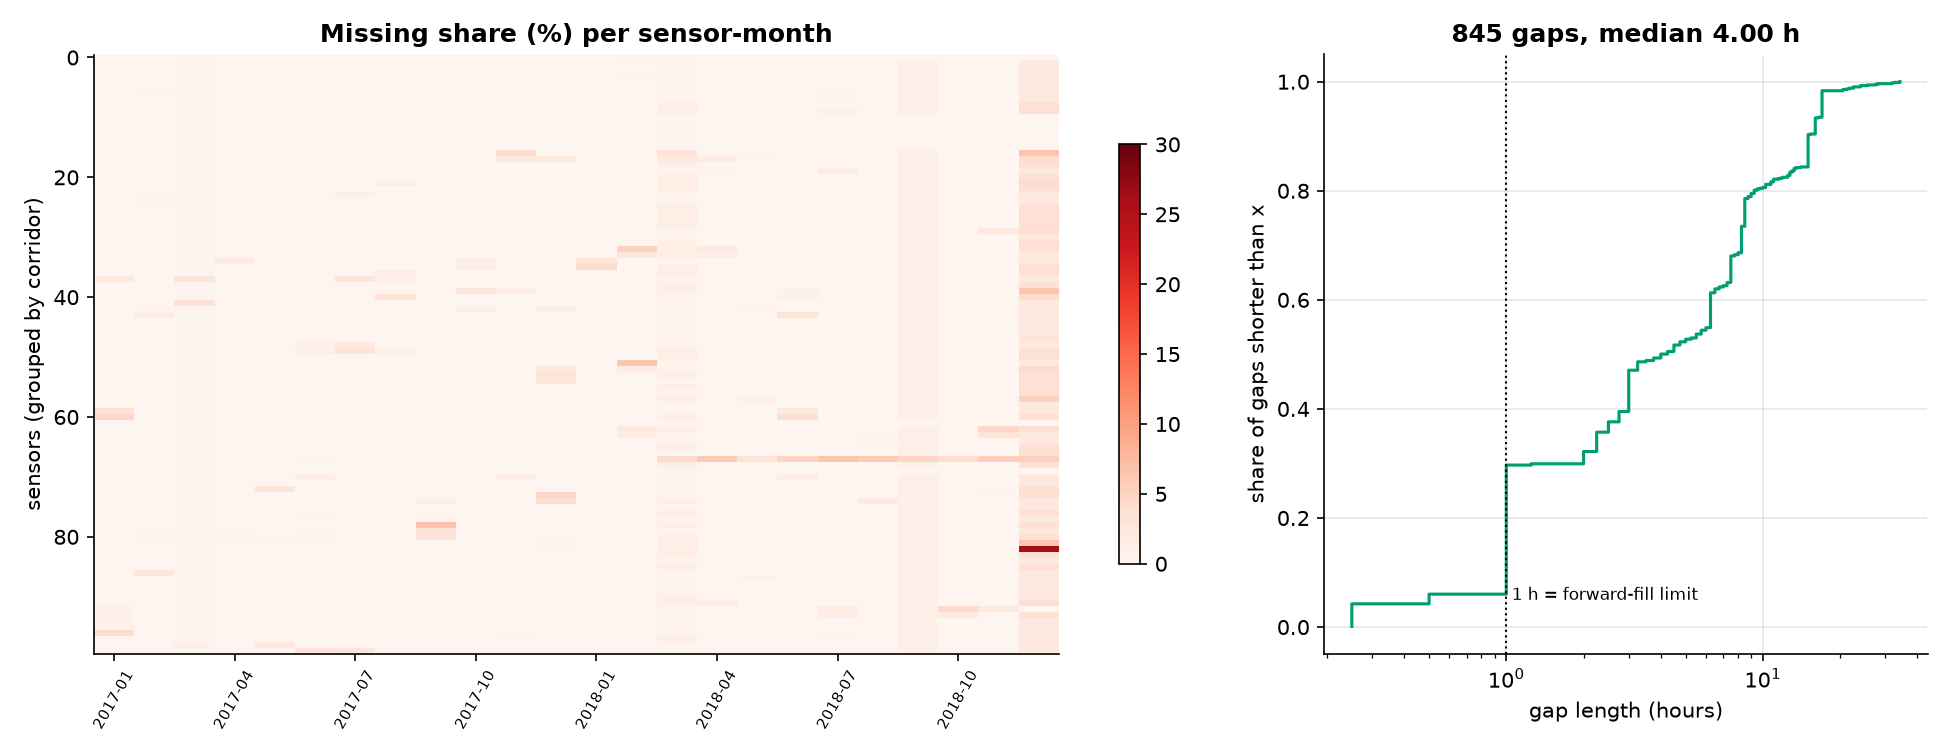
\includegraphics[width=\linewidth]{eda09_missing_data.png}
\caption{Missing data: when, where and for how long.}\label{fig:missing}
\end{figure}

% ============================================================================================================
\section{Preprocessing and sensor faults}
\paragraph{Faults (\code{src/cleaning.py}).} On the 5-minute readings we remove (set to missing) (i) runs of zeros of at least
two hours during the day (06:00--22:00), (ii) runs of identical non-zero values lasting at least two hours, and (iii)
values above 200 vehicles per lane per 5 minutes, which is physically impossible. Short zero dropouts below two hours are
\emph{kept}, because a live system would see them as well. A 15-minute value is the mean of the valid 5-minute readings
times three, if at least two of the three are valid.

\paragraph{Missing values (\code{src/imputation.py}).} Missing inputs are filled causally, using only earlier bins: first
the previous value (for at most one hour), then the value of the same bin one week earlier, then the median of the previous
week. Targets that are missing are never imputed, so no model is scored on an invented value.

\paragraph{Scale.} Every sensor has its own trailing scale: the mean of its last 7 days (the median of the last 28 days if that
is not available). The models predict the \emph{scaled} flow (flow divided by the scale), so one model serves a 2-lane road
and a 7-lane road; the prediction is multiplied by the scale again before scoring. All metrics are in vehicles per 15 minutes.

\paragraph{Template days.} Some PeMS detectors were filled with a weekly template: a day on which at least 90\% of the readings
equal the reading exactly 7 days earlier or later (\code{src/quality.py}). On such days there is nothing to forecast and
``same time last week'' is perfect. About \templateShare\% of all sensor-days are template days, and \nTemplateSensors{} sensors
(\templateSensorList) are template sensors on essentially every day (Figure~\ref{fig:template}). We keep these rows in the
main results, but report a second view, ``clean rows'' (template days removed, \keptPct\% of the 2019 rows kept), next to them.

\begin{figure}[H]\centering
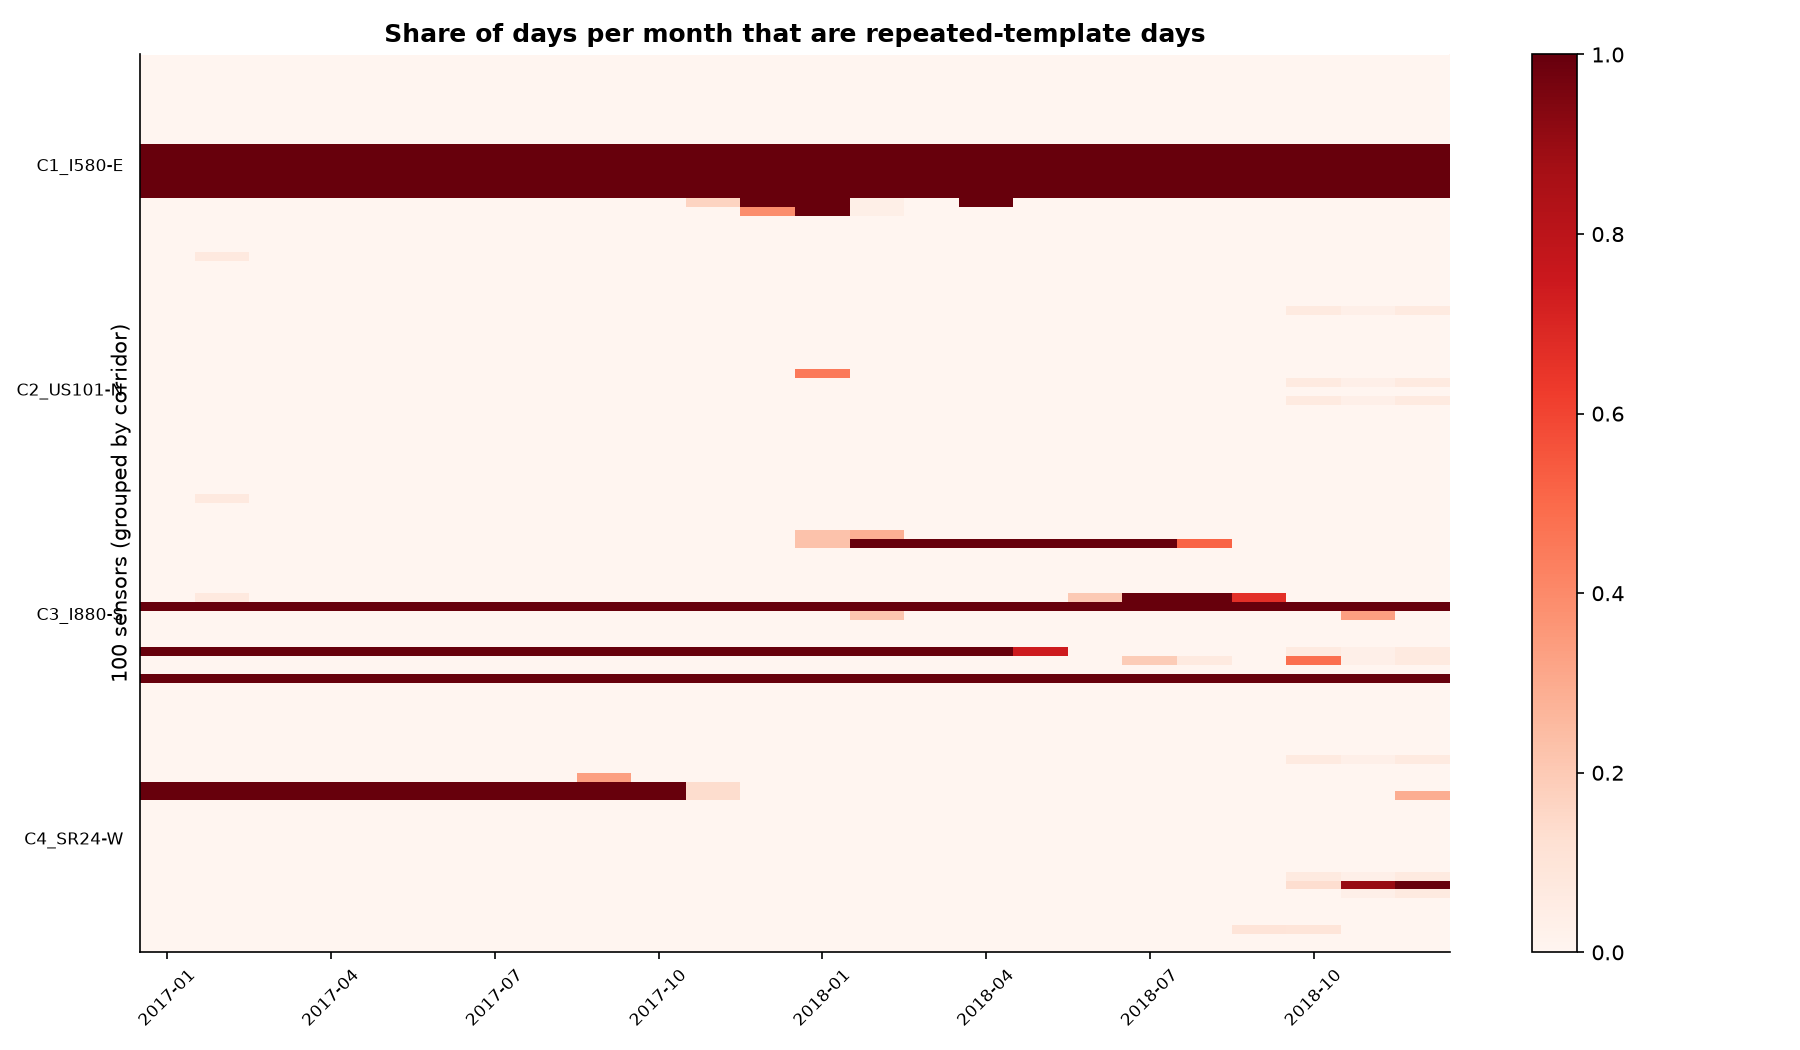
\includegraphics[width=0.9\linewidth]{eda13_template_days.png}
\caption{Share of days classified as template days, per sensor.}\label{fig:template}
\end{figure}

% ============================================================================================================
\section{Features, leakage prevention and split design}
\paragraph{Features.} Each row is one (sensor, forecast origin) pair with \nFeatures{} features in seven groups
(Table~\ref{tab:features}). All of them are computed from data before the origin only.

\begin{table}[H]\centering\small
\begin{tabular}{lrp{9.2cm}}
\toprule
Group & Count & Content \\
\midrule
Lags & 7 & flow now and 15, 30, 45, 60, 120 min ago; share of the last 3 h missing \\
Rolling & 6 & mean and std of the last 1 h and 3 h, 24 h mean, sensor scale (7-day mean) \\
Seasonal & 2 & same time last week; mean of the same time over the last 4 weeks \\
Calendar & 7 & time of day and weekday (sin, cos), month, holiday, weekend \\
Weather & 4 & precipitation, temperature, wind, rain in the last 3 h \\
Neighbours & 4 & flow of the sensor behind and ahead on the freeway, and whether they exist \\
Context & 1 & number of lanes \\
\textbf{Total} & \textbf{31} &  \\
\bottomrule
\end{tabular}

\caption{The feature groups.}\label{tab:features}
\end{table}

\paragraph{Split.} The split is chronological (Table~\ref{tab:splits}). Training ends on 2018-06-30, validation covers the second
half of 2018, and 2019 is the test year. The last four origins before each boundary are purged (one hour), so a target never
overlaps the next split. Each sensor keeps one origin in four (a fixed pattern) to limit correlated rows. Cold sensors appear
only in the test rows; their own history still feeds their lag features and scale, but warm sensors never use cold sensors
as neighbours.

\begin{table}[H]\centering\small
\begin{tabular}{lllrrr}
\toprule
Split & From & To & Rows (15 min) & Warm-sensor rows & Cold-sensor rows \\
\midrule
Train & 2017-01-29 & 2018-06-30 & 992,997 & 992,997 & 0 \\
Validation & 2018-07-01 & 2018-12-31 & 350,587 & 350,587 & 0 \\
Test & 2019-01-01 & 2019-12-31 & 868,158 & 693,469 & 174,689 \\
\bottomrule
\end{tabular}

\caption{Chronological split, 15-minute horizon (the 60-minute table has the same structure).}\label{tab:splits}
\end{table}

\paragraph{Leakage tests (\code{tests/}).} (1) \emph{Scramble the future:} all flow and weather data at and after a cut time are
replaced by random numbers and the feature table is rebuilt; every feature of every origin at or before the cut must be
identical. A positive control (scrambling the past) must change later features, which shows the test can fail.
(2) \emph{Live parity:} a function that is physically handed only the history before the origin rebuilds the 31 features for
every sensor and must reproduce the feature table row by row (837 rows $\times$ 32 columns); because it never sees the
future, parity shows that the table does not use it either. (3) The same function refuses a request for a future time. All six
leakage and parity tests pass, and five more unit tests cover the helper scripts (11 in total).

\paragraph{Test discipline.} Tuning and EDA use 2017--2018 only. After tuning, each model is refit on training plus validation with
the settings and tree count frozen, and predicts 2019 once; the writer refuses to overwrite an existing 2019 file. The
22 prediction files are fingerprinted (SHA-256) in \code{results/FROZEN.json}.

% ============================================================================================================
\section{Models, tuning and benchmark}
\paragraph{Baselines.} Persistence (the last reading), last week (same time one week earlier) and the four-week average of
that time. The strongest baseline on validation is used for the skill score: persistence at 15 minutes and the four-week average
at 60 minutes.

\paragraph{Models.} Ridge regression; PCA followed by Ridge (the number of components was chosen on validation and equals the
number of features, so it matches Ridge, i.e.\ no compression helps); a Decision Tree; a Random Forest; and the five boosting
variants AdaBoost, Gradient Boosting (scikit-learn), XGBoost, LightGBM and CatBoost. All models see the same rows and the same
31 features.

\paragraph{Tuning.} Each model is tuned on a 300{,}000-row month-stratified subset of the training period and scored on the
whole validation year; XGBoost, LightGBM and CatBoost stop early on validation (weighted so that the stopped quantity is the
raw-unit MAE). The search is small (a full grid for the cheap models, 4 to 8 random draws for the others), because the slow
models take hours; the selected settings are listed in Table~\ref{tab:tuning} in the appendix.

\paragraph{Metrics.} MAE and RMSE in vehicles per 15 minutes, WAPE, and \emph{skill}, the relative MAE reduction against the
best simple baseline. Confidence intervals come from a day-block bootstrap (1{,}000 draws): whole days are resampled, because
the errors within a day are strongly correlated.

\subsection{Results on the 2019 test year}
\begin{table}[H]\centering\small
\begin{tabular}{lrrrrr}
\toprule
Model & MAE & 95\% interval & RMSE & WAPE (\%) & Skill (\%) \\
\midrule
Persistence & 66.38 & {\small [65.57, 67.12]} & 99.01 & 7.24 & +0.0 \\
Last week & 91.78 & {\small [88.45, 95.43]} & 162.70 & 10.02 & -38.3 \\
4-week average & 78.44 & {\small [75.65, 81.43]} & 134.69 & 8.56 & -18.2 \\
\midrule
Ridge & 55.98 & {\small [55.32, 56.69]} & 85.28 & 6.11 & +15.7 \\
PCA + Ridge & 55.98 & {\small [55.32, 56.69]} & 85.28 & 6.11 & +15.7 \\
Decision Tree & 52.50 & {\small [51.88, 53.12]} & 82.16 & 5.73 & +20.9 \\
Random Forest & 49.55 & {\small [48.94, 50.19]} & 78.95 & 5.41 & +25.3 \\
AdaBoost & 51.12 & {\small [50.52, 51.76]} & 80.55 & 5.58 & +23.0 \\
Gradient Boosting & 50.78 & {\small [50.17, 51.42]} & 79.79 & 5.54 & +23.5 \\
XGBoost & 48.73 & {\small [48.08, 49.39]} & 77.85 & 5.32 & +26.6 \\
LightGBM & \textbf{48.63} & {\small [47.98, 49.28]} & \textbf{77.50} & \textbf{5.31} & +26.7 \\
CatBoost & 48.96 & {\small [48.33, 49.61]} & 77.66 & 5.34 & +26.2 \\
\bottomrule
\end{tabular}

\caption{Test results, 15 minutes ahead, all rows (868{,}158 rows, 100 sensors). Skill is the MAE reduction against persistence. The
interval is the 95\% day-block bootstrap interval of the MAE. Best value in bold.}\label{tab:h15}
\end{table}

\begin{table}[H]\centering\small
\begin{tabular}{lrrrrr}
\toprule
Model & MAE & 95\% interval & RMSE & WAPE (\%) & Skill (\%) \\
\midrule
Persistence & 142.01 & {\small [140.45, 143.46]} & 200.03 & 15.50 & -81.1 \\
Last week & 91.74 & {\small [88.44, 95.42]} & 162.68 & 10.01 & -17.0 \\
4-week average & 78.43 & {\small [75.61, 81.43]} & 134.61 & 8.56 & +0.0 \\
\midrule
Ridge & 75.26 & {\small [73.83, 76.72]} & 114.64 & 8.21 & +4.0 \\
PCA + Ridge & 75.26 & {\small [73.83, 76.72]} & 114.64 & 8.21 & +4.0 \\
Decision Tree & 67.12 & {\small [66.06, 68.16]} & 106.51 & 7.32 & +14.4 \\
Random Forest & 62.35 & {\small [61.36, 63.29]} & 99.77 & 6.80 & +20.5 \\
AdaBoost & 65.81 & {\small [64.76, 66.80]} & 103.95 & 7.18 & +16.1 \\
Gradient Boosting & 64.31 & {\small [63.34, 65.25]} & 101.17 & 7.02 & +18.0 \\
XGBoost & 61.29 & {\small [60.40, 62.18]} & 98.05 & 6.69 & +21.9 \\
LightGBM & \textbf{61.15} & {\small [60.27, 62.02]} & \textbf{97.57} & \textbf{6.67} & +22.0 \\
CatBoost & 61.58 & {\small [60.67, 62.49]} & 97.73 & 6.72 & +21.5 \\
\bottomrule
\end{tabular}

\caption{Test results, 60 minutes ahead, all rows. Skill is the MAE reduction against the four-week average.}\label{tab:h60}
\end{table}

\paragraph{Reading the tables.}
\begin{itemize}
\item \textbf{Models beat the baselines.} At 15 minutes LightGBM reaches an MAE of \lgbmMAEFifteen{} against \persMAEFifteen{} for persistence
(\lgbmSkillFifteen{}\% better). At 60 minutes persistence is poor (the traffic changes too much in an hour) and the best baseline is the
four-week average; LightGBM improves on it by \lgbmSkillSixty{}\% (MAE \lgbmMAESixty{}).
\item \textbf{Linear models are not enough.} Ridge, and with it PCA+Ridge, trail the tree ensembles clearly, especially at 60
minutes (MAE \ridgeMAESixty{}, only \ridgeSkillSixty{}\% better than the best baseline). The relationship between recent flow, the time of day and the
future flow is non-linear.
\item \textbf{Boosting and forests win.} The best group is LightGBM, XGBoost, CatBoost and Random Forest. A single Decision Tree
and the classic boosters (AdaBoost, Gradient Boosting) are clearly worse.
\item \textbf{The top of the ranking is a near tie.} The paired bootstrap (Table~\ref{tab:paired}) shows that LightGBM is better than
every other model on the same resampled days, but the margin over XGBoost is only \xgbGapFifteen{} MAE at 15 minutes and
\xgbGapSixty{} at 60 minutes (about 0.2\%), and CatBoost is within 0.4 vehicles. For practical purposes the three are equivalent;
the choice of LightGBM rests on a small but consistent advantage and on the shortest prediction path.
\end{itemize}

\begin{table}[H]\centering\small
\begin{tabular}{llrcr}
\toprule
h & Other model & MAE diff. & 95\% interval & LightGBM wins (\%) \\
\midrule
15 & XGBoost & 0.11 & [0.06, 0.15] & 100 \\
15 & CatBoost & 0.33 & [0.28, 0.37] & 100 \\
15 & Random Forest & 0.92 & [0.82, 1.03] & 100 \\
15 & Gradient Boosting & 2.15 & [2.05, 2.26] & 100 \\
15 & AdaBoost & 2.50 & [2.34, 2.65] & 100 \\
15 & Decision Tree & 3.87 & [3.74, 4.01] & 100 \\
15 & Ridge & 7.35 & [7.07, 7.67] & 100 \\
60 & XGBoost & 0.14 & [0.05, 0.23] & 100 \\
60 & CatBoost & 0.42 & [0.33, 0.52] & 100 \\
60 & Random Forest & 1.20 & [0.92, 1.47] & 100 \\
60 & Gradient Boosting & 3.15 & [2.87, 3.44] & 100 \\
60 & AdaBoost & 4.66 & [4.22, 5.10] & 100 \\
60 & Decision Tree & 5.97 & [5.57, 6.39] & 100 \\
60 & Ridge & 14.11 & [13.14, 15.17] & 100 \\
\bottomrule
\end{tabular}

\caption{Paired day-block bootstrap on the test year: MAE of the other model minus MAE of LightGBM (positive = LightGBM better), with
its 95\% interval and the share of the 1{,}000 resamples in which LightGBM is better. The interval reflects the variation
between days, not the training randomness (three LightGBM seeds differ by a standard deviation of 0.02 MAE).}\label{tab:paired}
\end{table}

\begin{figure}[H]\centering
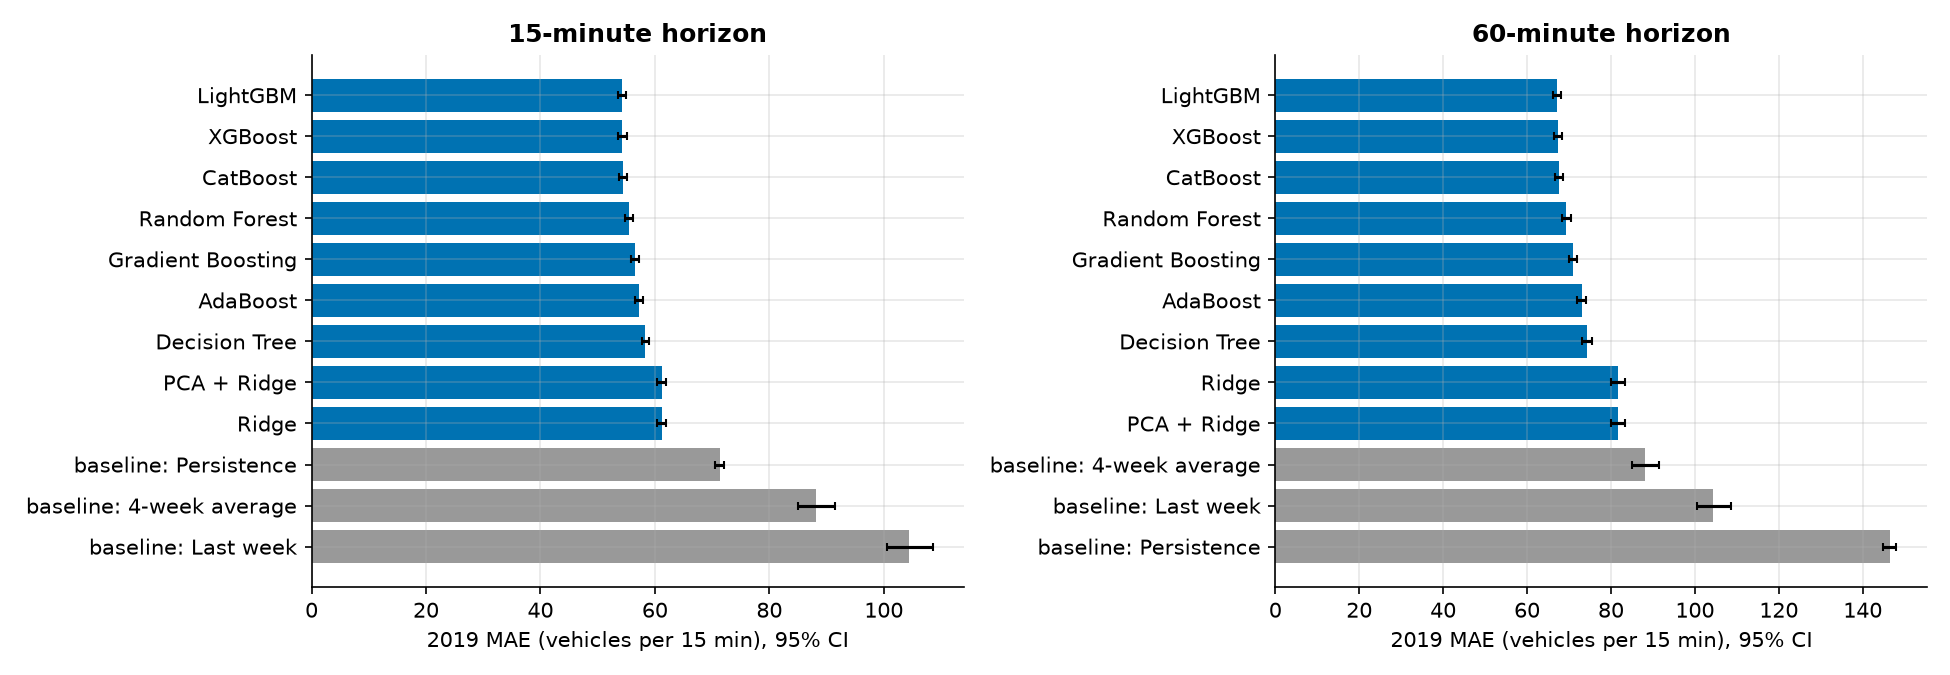
\includegraphics[width=\linewidth]{test_headline.png}
\caption{Headline results on the test year.}\label{fig:headline}
\end{figure}

\subsection{Clean rows and template sensors}
\begin{table}[H]\centering\small
\begin{tabular}{lrrrrr}
\toprule
Model & MAE & 95\% interval & RMSE & WAPE (\%) & Skill (\%) \\
\midrule
Persistence & 71.35 & {\small [70.50, 72.15]} & 104.53 & 7.73 & +0.0 \\
Last week & 104.35 & {\small [100.55, 108.54]} & 173.14 & 11.30 & -46.2 \\
4-week average & 88.11 & {\small [85.03, 91.51]} & 142.45 & 9.54 & -23.5 \\
\midrule
Ridge & 61.17 & {\small [60.45, 61.92]} & 90.63 & 6.63 & +14.3 \\
PCA + Ridge & 61.17 & {\small [60.45, 61.92]} & 90.63 & 6.63 & +14.3 \\
Decision Tree & 58.35 & {\small [57.67, 59.02]} & 87.65 & 6.32 & +18.2 \\
Random Forest & 55.51 & {\small [54.82, 56.19]} & 84.35 & 6.01 & +22.2 \\
AdaBoost & 57.18 & {\small [56.51, 57.85]} & 86.02 & 6.19 & +19.9 \\
Gradient Boosting & 56.52 & {\small [55.85, 57.19]} & 85.15 & 6.12 & +20.8 \\
XGBoost & 54.32 & {\small [53.62, 55.04]} & 83.11 & 5.88 & +23.9 \\
LightGBM & \textbf{54.20} & {\small [53.52, 54.89]} & \textbf{82.74} & \textbf{5.87} & +24.0 \\
CatBoost & 54.46 & {\small [53.79, 55.14]} & 82.89 & 5.90 & +23.7 \\
\bottomrule
\end{tabular}

\caption{Same as Table~\ref{tab:h15} but on the ``clean rows'' only (template days removed).}\label{tab:clean15}
\end{table}
Removing template days makes every number worse: LightGBM reaches an MAE of \lgbmCleanMAEFifteen{} (15 min) and \lgbmCleanMAESixty{}
(60 min) on clean rows. The \nTemplateSensors{} template sensors hold \tplRows\% of the test rows and are almost free to predict (WAPE
\tplWapeFifteen{}\% and \tplWapeSixty{}\%), while the other sensors score \otherWapeFifteen{}\% and \otherWapeSixty{}\% (MAE \otherMAEFifteen{} and \otherMAESixty{}).
The all-rows headline is therefore the honest measure of what a user of the app would see, and the clean-rows
view the fairer measure of traffic forecasting; both are reported.

\subsection{Warm and cold sensors}
\begin{table}[H]\centering\small
\begin{tabular}{lrrrrrr}
\toprule
Model & Warm & Cold & Gap & Warm & Cold & Gap \\
\midrule
Ridge & 5.99 & 6.59 & +0.60 & 8.09 & 8.70 & +0.61 \\
PCA + Ridge & 5.99 & 6.59 & +0.60 & 8.09 & 8.70 & +0.61 \\
Decision Tree & 5.61 & 6.23 & +0.62 & 7.20 & 7.82 & +0.61 \\
Random Forest & 5.29 & 5.91 & +0.62 & 6.69 & 7.28 & +0.59 \\
AdaBoost & 5.45 & 6.10 & +0.65 & 7.06 & 7.67 & +0.61 \\
Gradient Boosting & 5.42 & 6.02 & +0.60 & 6.90 & 7.48 & +0.58 \\
XGBoost & 5.20 & 5.81 & +0.61 & 6.56 & 7.21 & +0.65 \\
LightGBM & 5.19 & 5.80 & +0.61 & 6.55 & 7.19 & +0.64 \\
CatBoost & 5.22 & 5.83 & +0.61 & 6.60 & 7.22 & +0.62 \\
\bottomrule
\end{tabular}

\caption{WAPE (\%) on the test year for warm sensors (seen in training) and cold sensors (never seen). Left: 15 minutes. Right: 60 minutes.}\label{tab:warmcold}
\end{table}
Cold sensors are harder for every model (Table~\ref{tab:warmcold}), but only by about 0.6 WAPE points; the models transfer to new
locations because they predict a scaled flow and use the sensor's own recent history. Only 20 cold sensors exist, so this is a
small sample.

\subsection{Computational cost}
\begin{table}[H]\centering\small
\begin{tabular}{lrrrrrr}
\toprule
Model & Fit (s) & Predict (s/100k) & Size (MB) & Fit (s) & Predict (s/100k) & Size (MB) \\
\midrule
Ridge & 5 & 0.02 & 0.00 & 5 & 0.02 & 0.00 \\
PCA + Ridge & 1 & 0.03 & 0.01 & 1 & 0.03 & 0.01 \\
Decision Tree & 44 & 0.02 & 0.76 & 65 & 0.03 & 0.63 \\
Random Forest & 273 & 0.61 & 292.15 & 159 & 0.64 & 290.51 \\
AdaBoost & 7250 & 10.66 & 34.11 & 3799 & 1.30 & 24.67 \\
Gradient Boosting & 2480 & 0.68 & 1.03 & 2107 & 1.32 & 1.13 \\
XGBoost & 189 & 1.41 & 29.42 & 203 & 1.19 & 32.36 \\
LightGBM & 147 & 5.07 & 17.40 & 233 & 6.49 & 20.76 \\
CatBoost & 640 & 0.12 & 8.47 & 388 & 0.18 & 8.47 \\
\bottomrule
\end{tabular}

\caption{Fit time on training plus validation rows (1.34 million rows, CPU), prediction time per 100{,}000 rows and model size.}\label{tab:cost}
\end{table}
Ridge and PCA+Ridge are essentially free; the boosted models need minutes (XGBoost, LightGBM) to hours (scikit-learn Gradient Boosting
and AdaBoost). LightGBM, XGBoost and CatBoost combine the best accuracy with prediction speeds of a few seconds per 100{,}000 rows
and model sizes of tens of megabytes (Random Forest: about 290 MB).

% ============================================================================================================
\section{Analysis A: feature ablation}
Each of the seven feature groups is removed in turn, and every model is refit on the same training rows (300{,}000 for most
models, fewer for the slowest) and compared with its own full-feature reference. Table~\ref{tab:abl15} shows the relative increase
in validation MAE (positive = the group helps). For LightGBM, a cumulative build-up in a fixed order is also run
(Figure~\ref{fig:abl}).

\begin{table}[H]\centering\small
\begin{tabular}{lrrrrrrr}
\toprule
Model & Lags & Rolling & Seasonal & Calendar & Weather & Neighbours & Context \\
\midrule
Ridge & +13.4 & +0.5 & +4.4 & +1.3 & -0.0 & -0.1 & +0.0 \\
PCA + Ridge & +13.4 & +0.5 & +4.4 & +1.3 & -0.0 & -0.1 & +0.0 \\
Decision Tree & +12.0 & +0.1 & +3.7 & +0.9 & -0.1 & -0.1 & +0.0 \\
Random Forest & +10.3 & +1.0 & +3.4 & +1.6 & -0.1 & -0.3 & -0.0 \\
AdaBoost & +10.5 & +0.8 & +5.0 & +1.3 & -0.1 & -0.1 & -0.1 \\
Gradient Boosting & +8.4 & +0.8 & +2.4 & +3.2 & -0.1 & -0.2 & +0.0 \\
XGBoost & +5.2 & +1.2 & +2.1 & +4.4 & -0.4 & +0.1 & +0.2 \\
LightGBM & +5.0 & +1.1 & +2.0 & +4.8 & -0.5 & -0.0 & +0.1 \\
CatBoost & +4.4 & +1.2 & +2.0 & +4.5 & -0.5 & +0.1 & +0.2 \\
\bottomrule
\end{tabular}

\caption{Increase in validation MAE (\%) when a feature group is removed, 15 minutes ahead.}\label{tab:abl15}
\end{table}

\begin{figure}[H]\centering
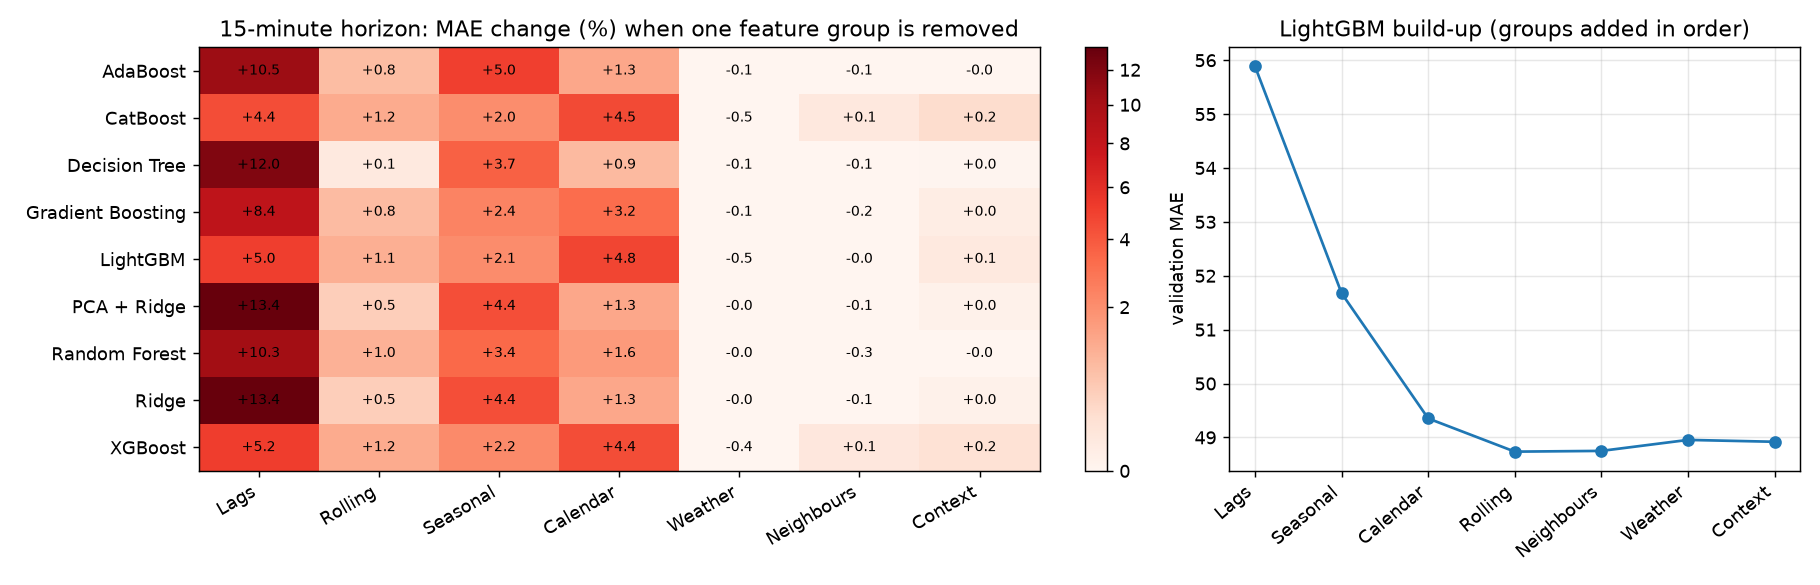
\includegraphics[width=\linewidth]{ablation_h15.png}
\caption{Ablation at 15 minutes: group removal for all models and cumulative build-up for LightGBM.}\label{fig:abl}
\end{figure}

\begin{table}[H]\centering\small
\begin{tabular}{lrrrrrrr}
\toprule
Model & Lags & Rolling & Seasonal & Calendar & Weather & Neighbours & Context \\
\midrule
Ridge & +4.2 & +0.9 & +29.6 & +1.8 & -0.1 & +0.3 & +0.0 \\
PCA + Ridge & +4.2 & +0.9 & +29.6 & +1.8 & -0.1 & +0.3 & +0.0 \\
Decision Tree & +4.7 & +0.3 & +8.4 & +2.6 & -0.1 & -0.0 & -0.0 \\
Random Forest & +3.7 & +1.8 & +9.1 & +4.2 & -0.3 & -0.8 & -0.2 \\
AdaBoost & +3.5 & +0.7 & +8.5 & +2.6 & -0.2 & -0.1 & -0.1 \\
Gradient Boosting & +2.0 & +0.8 & +10.9 & +4.2 & -0.5 & -0.6 & +0.0 \\
XGBoost & +2.2 & +2.3 & +6.8 & +7.6 & -0.8 & +0.4 & +0.4 \\
LightGBM & +2.0 & +2.4 & +6.6 & +8.1 & -1.0 & +0.2 & +0.4 \\
CatBoost & +1.9 & +2.4 & +7.6 & +7.6 & -0.6 & +0.3 & +0.5 \\
\bottomrule
\end{tabular}

\caption{Same as Table~\ref{tab:abl15}, 60 minutes ahead.}\label{tab:abl60}
\end{table}

\paragraph{Interpretation.}
\begin{itemize}
\item \textbf{At 15 minutes the recent readings and the calendar matter most.} Removing the lags raises the error of single trees, forests and
linear models by 10--13\%, but only by about 5\% for the boosted models, because the rolling means, the seasonal values and the calendar partly
replace them. For LightGBM, XGBoost and CatBoost the calendar group is as important as the lags (+\ablCalLgbm\% against +\ablLagsLgbm\% for LightGBM): they learn
the typical profile of each time of the week. The seasonal group (same time last week) adds \ablSeasLgbm\% for LightGBM.
\item \textbf{At 60 minutes the weekly pattern takes over.} Removing the calendar costs LightGBM 8.1\% and the seasonal group 6.6\%, while the lags cost only
2.0\%: an hour ahead, the current reading says less than what usually happens at that time. The linear model depends most on
the seasonal group (+29.6\%), because sine and cosine terms give it only a smooth, single-harmonic daily profile.
\item \textbf{Weather adds no accuracy.} Removing the weather group changes the error of the boosted models by $-0.4$ to $-1.0$\%, i.e.\ the models are
very slightly \emph{better} without it. Rain does raise the error in the error analysis, but the calendar already captures most of the weather
signal (rain is seasonal) and an hourly reanalysis value at one point per corridor is too coarse to add more.
\item \textbf{Neighbours and the lane count are neutral} (within $\pm$0.8\%): a sensor's own history already contains most of its local state, and
the lane count is presumably already reflected in each sensor's scale.
\item \textbf{PCA does not help.} PCA with all 31 components equals Ridge, and fewer components were never better on validation
(Figure~\ref{fig:pca}), so the features are not redundant enough for dimensionality reduction to pay off.
\end{itemize}

\begin{figure}[H]\centering
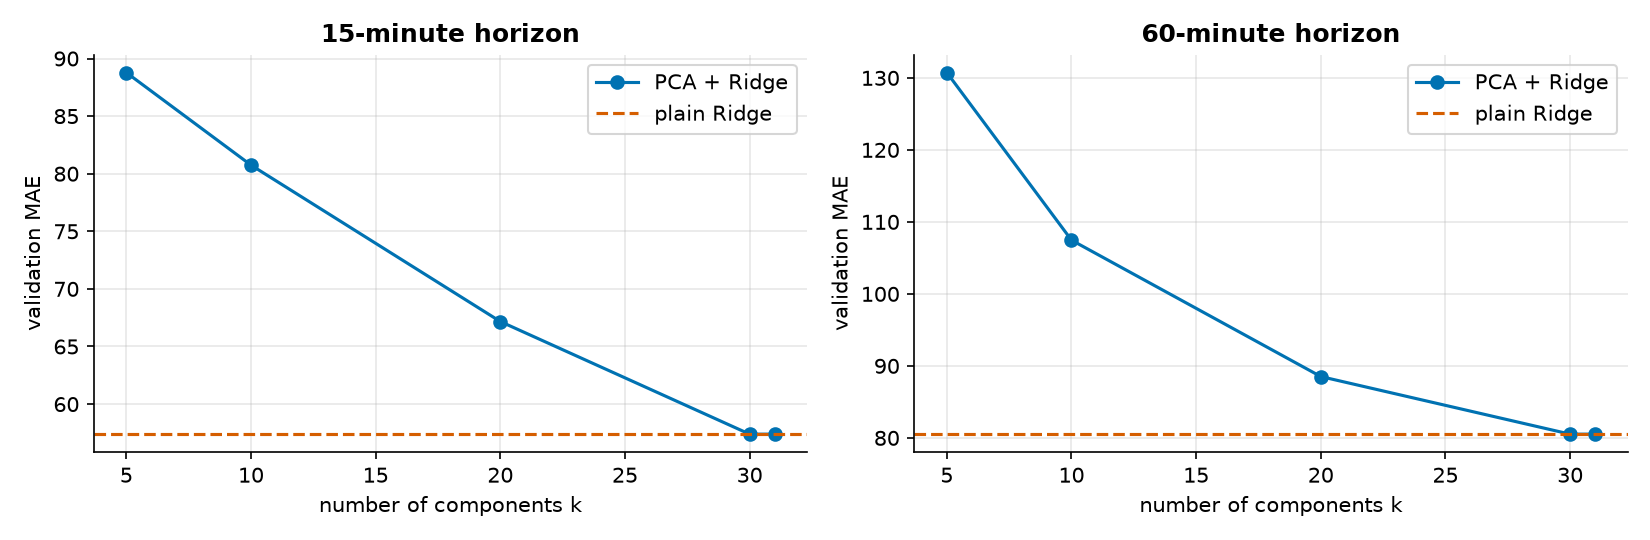
\includegraphics[width=0.7\linewidth]{model_pca_curve.png}
\caption{Validation error of PCA+Ridge as a function of the number of components.}\label{fig:pca}
\end{figure}

% ============================================================================================================
\section{Analysis D: robustness and sensitivity}
Models are fitted once on all training rows with their frozen settings and then stressed on the \emph{validation} year (the test
year is not used). Four experiments: (i) multiplicative Gaussian noise (5, 10, 20\%) on the five lag readings; (ii) the latest
reading missing for 10, 30 or 50\% of the rows, replaced by the reading before it (what a deployed system would do);
(iii) a reduced training history of 1, 3, 6 or 12 months; (iv) a random half of the warm sensors is used for training and
the model is scored on the other half, which it has never seen. The same random half and noise stream are used for every
model. The two slowest models (Gradient Boosting, AdaBoost) are refit on capped training rows (150{,}000 and 100{,}000), and the history
experiment is run for the three cheapest models only (Ridge, Decision Tree, LightGBM).

\begin{table}[H]\centering\small
\begin{tabular}{lrrrrrrrr}
\toprule
Model & Noise 10\% & Miss. 30\% & Unseen & 3 mo & Noise 10\% & Miss. 30\% & Unseen & 3 mo \\
\midrule
Ridge & +28.0 & +6.5 & +0.1 & +1.7 & +8.8 & +2.2 & +0.7 & +0.5 \\
PCA + Ridge & +27.8 & +6.4 & +0.1 & -- & +8.8 & +2.1 & +0.7 & -- \\
Decision Tree & +28.3 & +6.8 & +2.6 & +8.1 & +8.4 & +1.9 & +3.5 & +11.9 \\
Random Forest & +23.2 & +6.7 & +2.0 & -- & +6.3 & +1.7 & +3.8 & -- \\
AdaBoost & +27.4 & +6.6 & +1.5 & -- & +5.9 & +1.3 & +2.0 & -- \\
Gradient Boosting & +22.7 & +6.0 & +1.3 & -- & +5.7 & +1.4 & +3.1 & -- \\
XGBoost & +29.0 & +6.4 & +4.4 & -- & +10.3 & +1.9 & +8.7 & -- \\
LightGBM & +26.0 & +6.3 & +3.3 & +8.7 & +8.8 & +2.0 & +8.1 & +13.3 \\
CatBoost & +26.9 & +6.5 & +3.1 & -- & +8.6 & +2.0 & +6.7 & -- \\
\bottomrule
\end{tabular}

\caption{Increase in validation MAE (\%) under stress. Noise 10\%: multiplicative noise on the lag readings. Miss.\ 30\%: the latest reading
is missing in 30\% of the rows. Unseen: trained on half of the sensors, scored on the other half. 3 mo: trained on the last three
months only. Left: 15 minutes, right: 60 minutes.}\label{tab:robust}
\end{table}

\begin{figure}[H]\centering
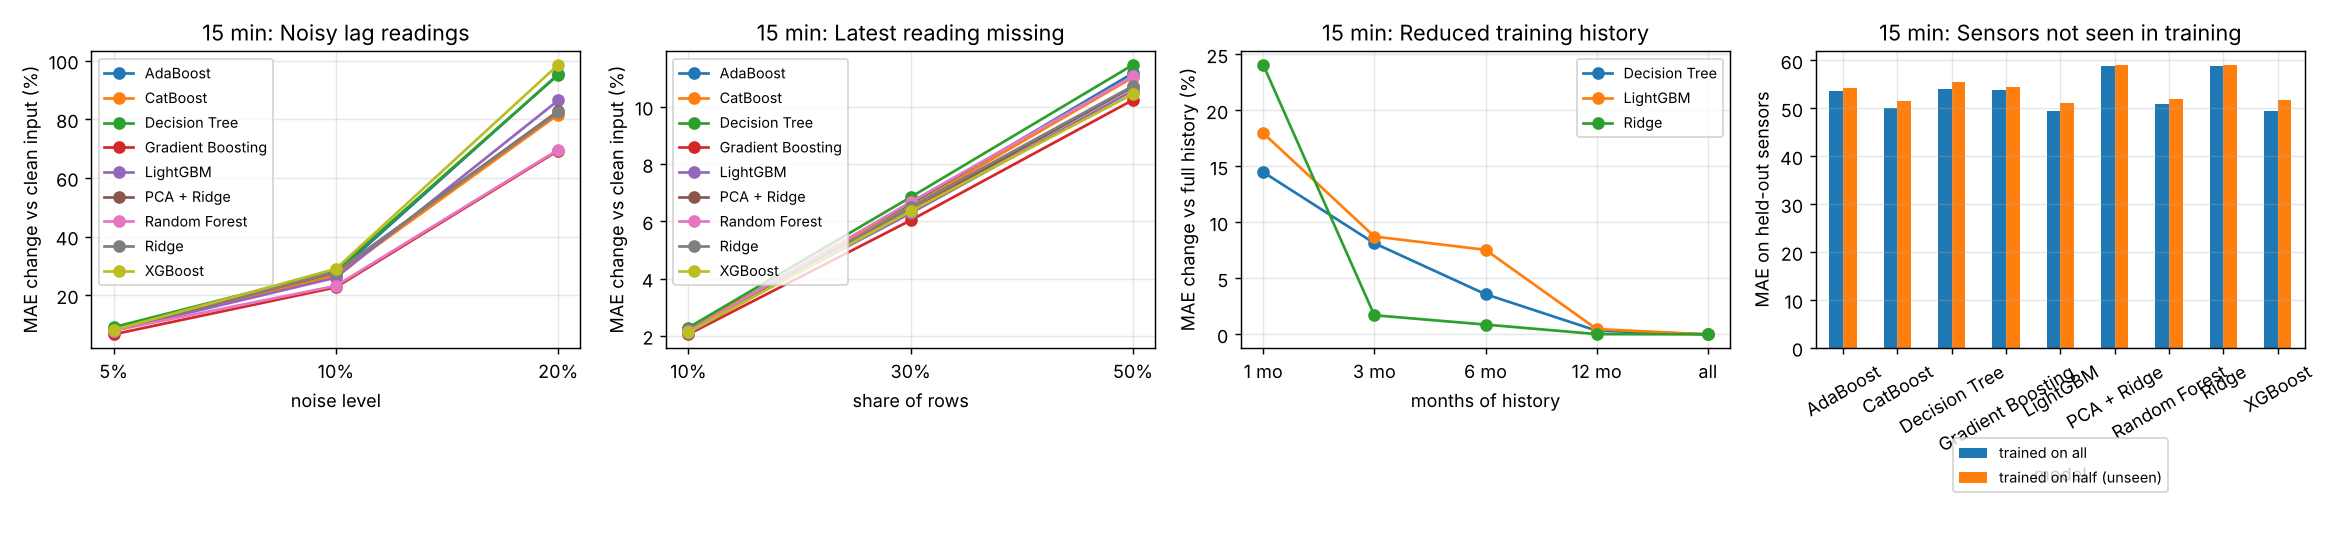
\includegraphics[width=\linewidth]{robust_h15.png}
\caption{Robustness at 15 minutes.}\label{fig:rob15}
\end{figure}

\paragraph{Interpretation.}
\begin{itemize}
\item \textbf{Noise on the recent readings is the most damaging stress.} With 10\% multiplicative noise on the lags, the 15-minute MAE rises by 23--29\% for every
model, and by 69--99\% with 20\% noise. At 60 minutes the effect is much smaller (6--10\% at 10\% noise) because the lags matter less an hour ahead (Analysis A).
Gradient Boosting and Random Forest (and AdaBoost at 60 minutes), which average many trees, are the least sensitive; XGBoost is the most sensitive. The noise is applied to the lag
readings only (the rolling and seasonal features stay clean), so this under-states the harm of a really noisy sensor.
\item \textbf{A missing latest reading is mild when it is carried forward.} The error grows roughly in proportion to the share of affected rows (+2\%, +6--7\% and +10--11\%
for 10, 30 and 50\% of the rows at 15 minutes, +0.4 to +3.7\% at 60 minutes) and is almost the same for all models. A deployed system can therefore survive short
outages of the latest reading by carrying the previous value forward, as the app does.
\item \textbf{Unseen sensors cost little, and flexible models pay most.} Trained on half of the warm sensors and scored on the other half, the MAE rises by 1.3 to 4.4\%
at 15 minutes and 2 to 8.7\% at 60 minutes, most for XGBoost, LightGBM and CatBoost and least for the linear models (0.1 to 0.7\%). Even with half of the sensors, the boosted models
stay far ahead of Ridge (about 64 against 78 at 60 minutes). This test mixes two effects (unseen sensors and half as many training rows), and the real cold
sensors in the test year show a similar small gap (Table~\ref{tab:warmcold}).
\item \textbf{Flexible models need about a year of history.} LightGBM loses 0.5--0.8\% when trained on 12 instead of 18 months, about 9\% (15 min) and 13\% (60 min) with 3 months, and
18\% and 27\% with one month; a decision tree behaves similarly. Ridge hardly changes with 3 months or more, because it only has a few weights to learn. A model that must learn the weekly and seasonal
pattern needs at least a full year.
\end{itemize}
Taken together: a deployed system should check the quality of the latest readings (noise matters), can carry forward missing ones, can be applied to new sensors on the same
kind of freeway at a small cost, and should be trained on at least a year of data. (Ridge and PCA+Ridge are the same model here, since PCA keeps all 31 components. The feature \texttt{mean\_1h} is exactly the average of four lag columns, so the
weight on that direction is set by rounding. It does not matter on clean data, but it changes the response to noise on the lags, so the two linear models are fitted in
double precision in this experiment, where they agree.)

% ============================================================================================================
\section{Analysis E: error analysis}
All models are scored on the test year, segmented by peak hours, weekday/weekend/holiday, rain, the size of the change since the
last reading, the flow level, warm or cold sensors, hour of day and individual sensor (LightGBM in Table~\ref{tab:segments}; the notebook
has all nine models).

\begin{table}[H]\centering\small
\begin{tabular}{llrr}
\toprule
Segment & Level & 15 min & 60 min \\
\midrule
Peak & off-peak & 5.43 & 6.85 \\
 & peak & 5.04 & 6.29 \\
\midrule
Weekend & weekday & 5.35 & 6.69 \\
 & weekend & 5.11 & 6.39 \\
 & holiday & 6.04 & 8.62 \\
\midrule
Rain & dry & 5.25 & 6.58 \\
 & rain & 5.87 & 7.61 \\
\midrule
Change since last reading & Q1 steady & 3.06 & 4.52 \\
 & Q2 & 3.38 & 5.28 \\
 & Q3 & 4.47 & 6.64 \\
 & Q4 sudden & 9.55 & 10.36 \\
\midrule
Level & low flow & 8.18 & 11.17 \\
 & mid flow & 5.73 & 7.09 \\
 & high flow & 4.24 & 5.19 \\
\midrule
Role & warm & 5.19 & 6.55 \\
 & cold & 5.80 & 7.19 \\
\bottomrule
\end{tabular}

\caption{WAPE (\%) of LightGBM on the test year, by segment.}\label{tab:segments}
\end{table}

\begin{figure}[H]\centering
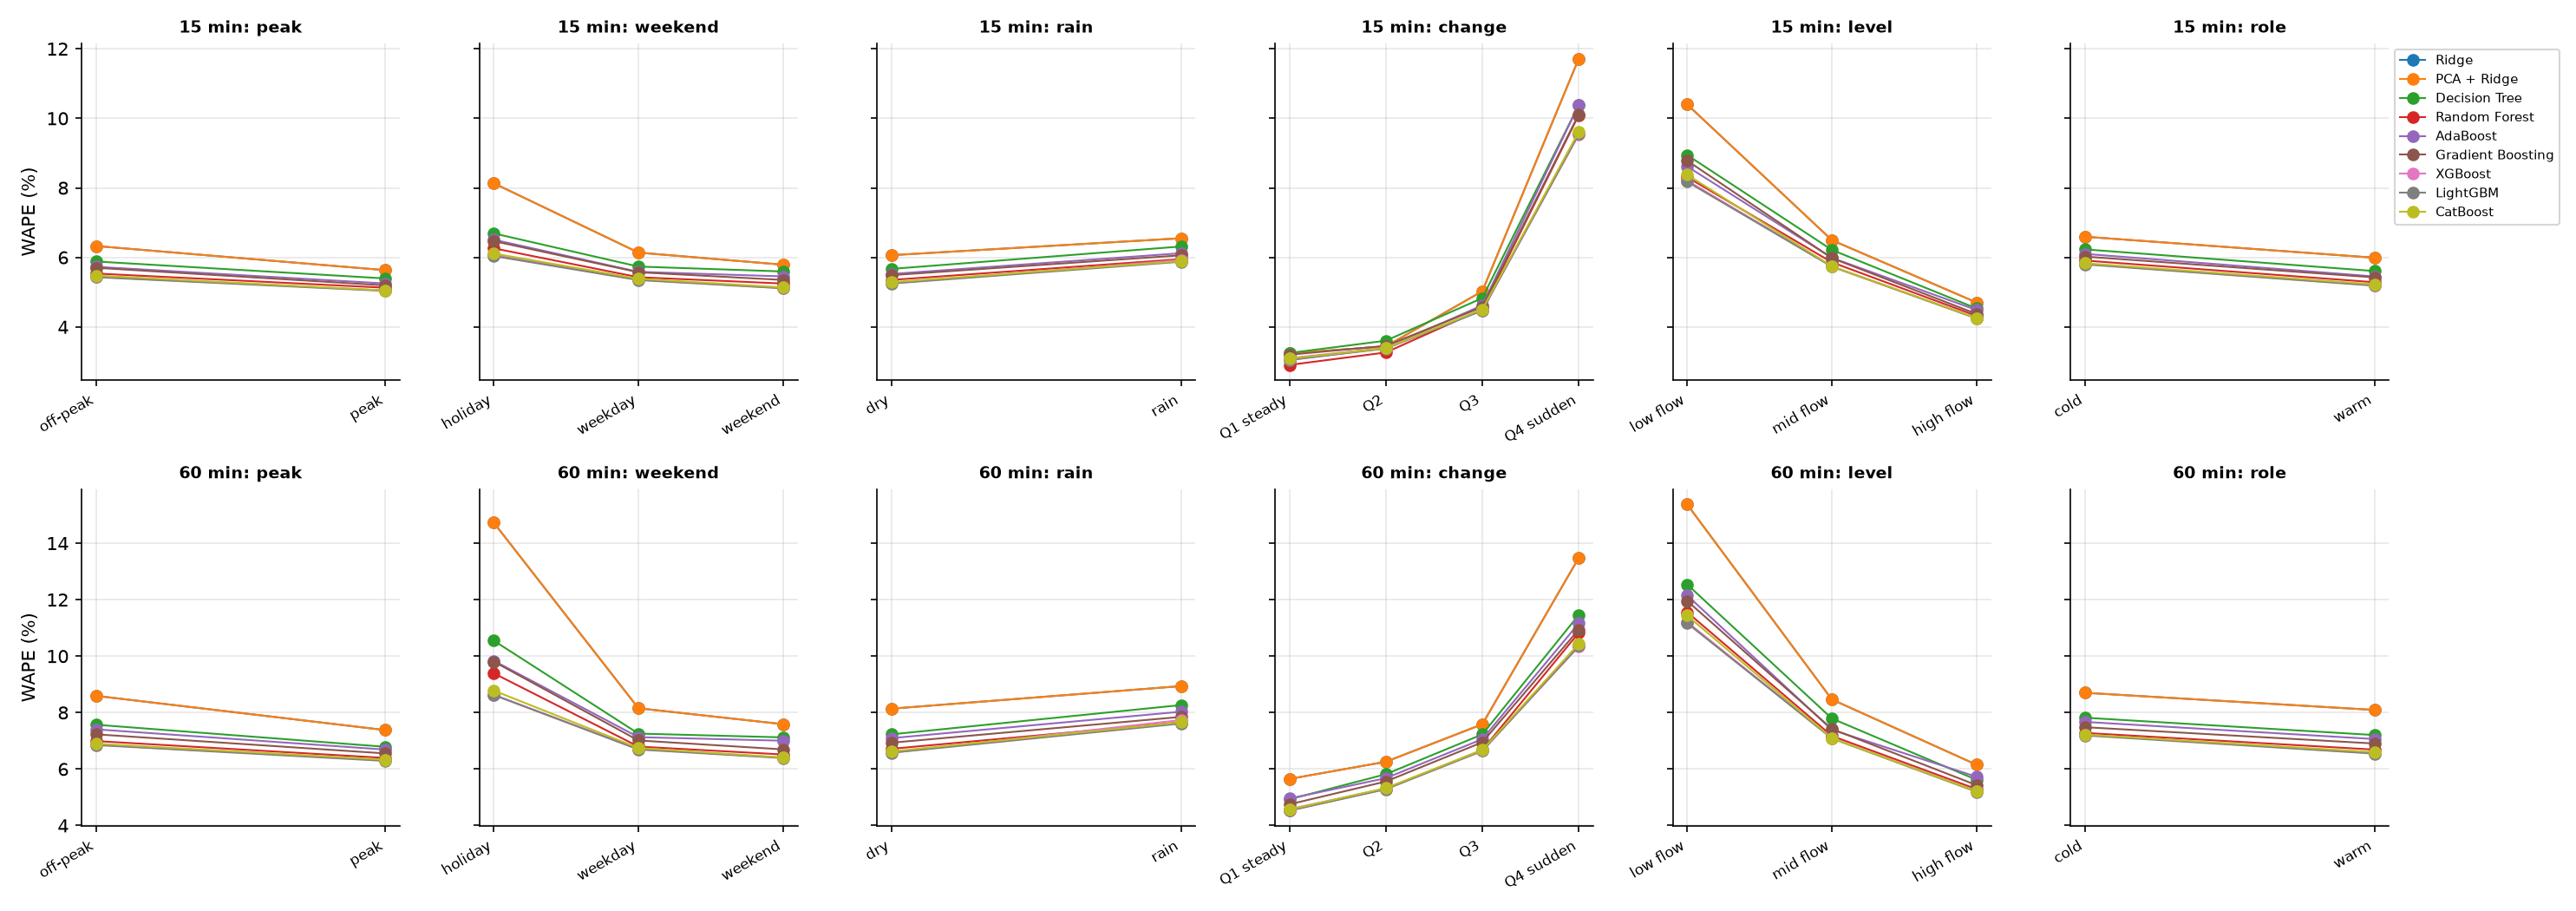
\includegraphics[width=\linewidth]{err_segments_test.png}
\caption{WAPE by segment for all nine models, test year.}\label{fig:errseg}
\end{figure}

\paragraph{Findings.}
\begin{itemize}
\item \textbf{Sudden changes are the main driver of error.} The quartile of rows with the smallest move since the last reading scores
\chgSteadyFifteen{}\% WAPE (15 min), the quartile with the largest move \chgSuddenFifteen{}\%; at 60 minutes the values are \chgSteadySixty{}\%
and \chgSuddenSixty{}\%.
\item \textbf{Peak hours are not harder than off-peak hours} in relative terms, because WAPE divides by larger flows. Low-flow rows are about
twice as hard as high-flow rows (\lowFlowFifteen{}\% against \highFlowFifteen{}\% at 15 minutes), since a fixed error is a larger share of a small flow.
\item \textbf{Holidays and rain are the weak segments.} Holidays score \holidayFifteen{}\% against \weekdayFifteen{}\% on weekdays at 15 minutes
(\holidaySixty{}\% against \weekdaySixty{}\% at 60 minutes). Rain scores \rainFifteen{}\% against \dryFifteen{}\% dry (\rainSixty{}\% against \drySixty{}\%). Both are
rare, so the models have fewer examples.
\item \textbf{The models fail on the same rows.} The absolute errors of the boosted models correlate at 0.96 to 0.98, and the
per-sensor ranking of difficulty is nearly identical for all models (Spearman 0.97 to 1.00). The hard rows are hard because of the
data, not because of one model.
\item \textbf{A few rows dominate.} The worst 1\% of rows carries about 8\% of the total absolute error, mostly in the quartile of the largest sudden
changes. These are feed outages: on 2019-09-20 at 12:00, 18 of the 100 sensors read exactly 0 and 29 were below 20\% of their usual flow;
on 2019-09-18 at 11:15, 23 sensors were below 20\%. Four separate freeways cannot collapse in the same quarter of an hour, so no feature
can predict these rows, and the models were not changed because of them.
\item \textbf{One sensor has uncleaned faults.} Sensor 719 (SR-24 W) has isolated night-time spikes (2.5\% of its night bins above 1{,}000 vehicles per 15 minutes) that
the cleaning rule does not flag, because the limit is per lane.
\end{itemize}

\begin{figure}[H]\centering
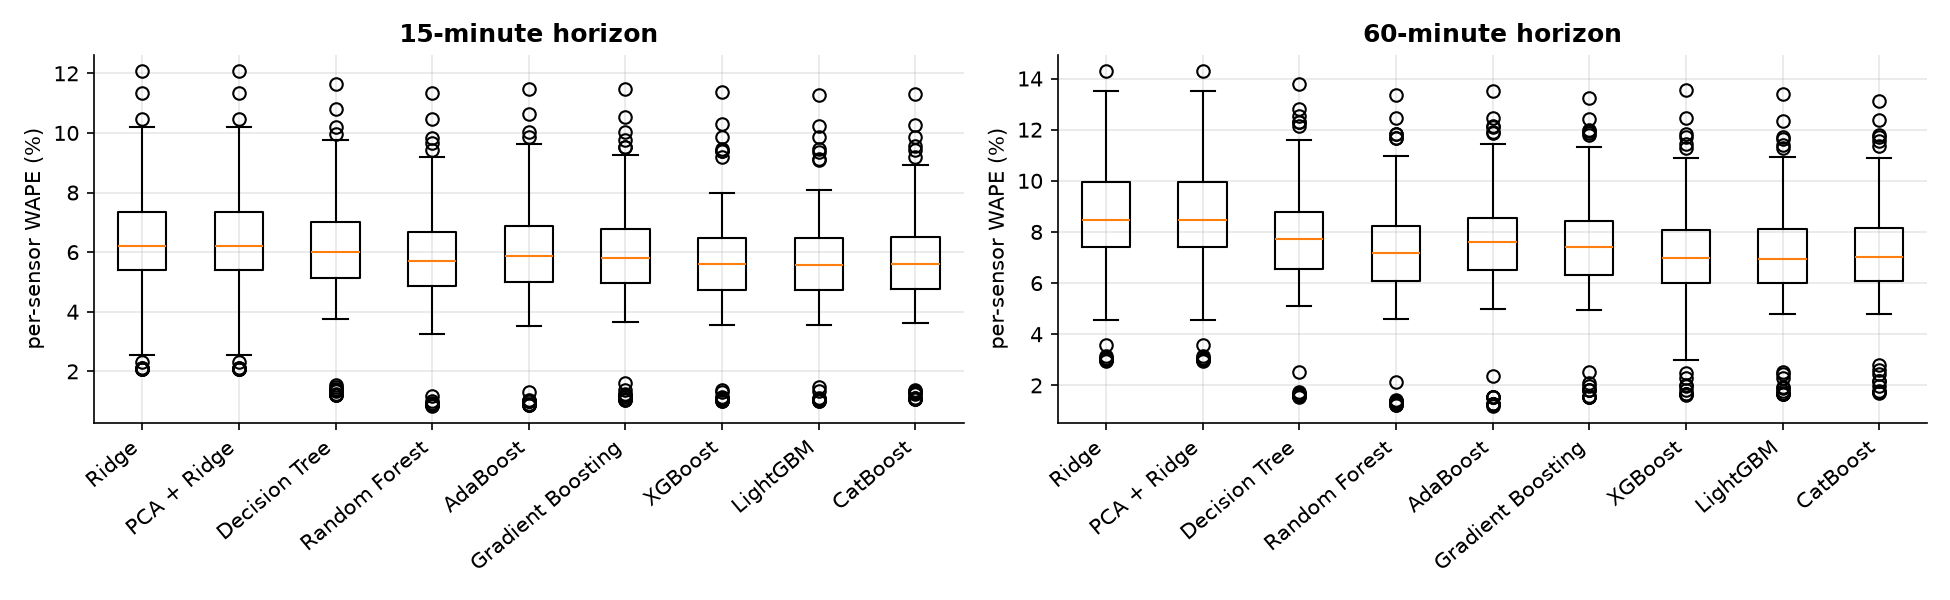
\includegraphics[width=\linewidth]{err_per_sensor_test.png}
\caption{WAPE by sensor, test year. The very easy sensors on the left are the template sensors.}\label{fig:errsensor}
\end{figure}

% ============================================================================================================
\section{Comparison with published results}
The LargeST paper \cite{largest} benchmarks graph neural networks on the whole Greater Bay Area subset (2{,}352 sensors, 2019 only, 12 steps
of 15 minutes in and out). Table~\ref{tab:published} sets our LightGBM next to their numbers. The comparison is
\emph{not} like-for-like: their sensors are all 2{,}352 detectors including quiet ones, while ours are 100 well-instrumented corridor
sensors that carry far more traffic (mean flow about 916 vehicles per 15 minutes), so the absolute MAE is not comparable. We therefore
compare scale-free quantities: the error relative to persistence (their ``Historical Last'') and the MAPE. Our 60-minute horizon lies between
their 45 and 90 minute columns.

\begin{table}[H]\centering\small
\begin{tabular}{llrrrr}
\toprule
Horizon & Method & MAE & MAPE (\%) & MAE / persist. & MAPE / persist. \\
\midrule
45 min & Historical Last (persistence) & 32.57 & 22.8 & 1.00 & 1.00 \\
45 min & LSTM & 20.38 & 15.5 & 0.63 & 0.68 \\
45 min & DCRNN & 18.71 & 14.7 & 0.57 & 0.65 \\
45 min & Graph WaveNet & 17.85 & 13.9 & 0.55 & 0.61 \\
45 min & D2STGNN (best at H3) & 17.54 & 12.1 & 0.54 & 0.53 \\
90 min & Historical Last (persistence) & 53.79 & 43.0 & 1.00 & 1.00 \\
90 min & LSTM & 27.56 & 23.5 & 0.51 & 0.55 \\
90 min & DCRNN & 23.06 & 20.4 & 0.43 & 0.48 \\
90 min & Graph WaveNet & 21.11 & 17.8 & 0.39 & 0.41 \\
90 min & D2STGNN (best at H3) & 20.92 & 14.9 & 0.39 & 0.35 \\
15 min & Ours: LightGBM & 48.63 & 9.6 & 0.73 & 0.82 \\
15 min & Ours: persistence & 66.38 & 11.8 & 1.00 & 1.00 \\
60 min & Ours: LightGBM & 61.15 & 14.2 & 0.43 & 0.46 \\
60 min & Ours: persistence & 142.01 & 30.7 & 1.00 & 1.00 \\
\bottomrule
\end{tabular}

\caption{LargeST GBA results (Table 2 of \cite{largest}) and ours. ``/ persist.'' divides the error by the error of the persistence
baseline at the same horizon. Our MAPE excludes rows whose true flow is zero; their treatment of zeros is not stated.}\label{tab:published}
\end{table}

At 60 minutes our LightGBM has a relative error of \ratioSixty{} against persistence and a MAPE of \mapeSixty\% (persistence: \mapePersSixty\%), which is
the range the published graph networks reach between 45 and 90 minutes (MAE ratio 0.54 to 0.39 for the best of them). Our persistence MAPE lies between
theirs at 45 minutes (22.8\%) and 90 minutes (43.0\%), which suggests the data behave alike. We read this as: a feature-engineered
gradient-boosting model on a sensor's own history, its neighbours and calendar variables reaches the same range as graph networks for
this horizon, at a fraction of the training cost, but we have not run those networks ourselves, so we do not claim to beat them.
In the same spirit, a PCA plus LightGBM solution won second place in the core track of the Traffic4cast 2022 traffic-forecasting challenge \cite{traffic4cast}.

% ============================================================================================================
\section{User interface}
The Streamlit application (\code{app/streamlit\_app.py}) is connected to the trained pipeline. The user chooses a horizon, a corridor, a sensor
and a date and time (quick examples are provided). The app then rebuilds the 31 features from the history \emph{before} that time through the
same function that the parity test checks, predicts with LightGBM, and shows:
\begin{itemize}
\item the forecast with an 80\% interval taken from the validation error quantiles, next to the latest reading and, if the time lies in the past,
the actual value;
\item the recent flow and the forecast on a time axis, with the baselines, and a view of the whole corridor;
\item a per-prediction explanation (LightGBM contributions per feature);
\item a stress test: the latest reading can be declared missing, and noise can be added to the recent readings, which shows the effect of
Analysis D interactively;
\item the benchmark tables.
\end{itemize}
Sensors and origins outside the available history produce a clear message instead of a forecast.
\todo{insert two screenshots of the app}

% ============================================================================================================
\section{Limitations and conclusions}
\paragraph{Limitations.}
\begin{itemize}
\item \textbf{Template sensors} flatter the all-rows results (WAPE about 1\% on eight sensors); the clean-rows view is reported next to it.
\item \textbf{Feed outages and sensor faults.} Short dropouts are kept, because a live system sees them, and they dominate the largest errors; sensor 719 has unflagged spikes.
\item \textbf{Small tuning budget.} Searches were small and several best settings sit at the edge of the grid (the iteration caps of CatBoost at 2{,}000 and of
Gradient Boosting at 300 trees were reached). The top three models are within about 0.3 MAE, so their order could change with wider tuning; the gap to the
other models is large. We measured the headroom on validation only (Appendix~\ref{app:sens}): a wider random search for LightGBM, XGBoost and CatBoost lowers the validation MAE
by 0.3 to 0.4\% (LightGBM, XGBoost at 15 minutes), 0.6\% (XGBoost at 60 minutes) and 0.9 to 1.2\% (CatBoost, which also hits its iteration cap). Wider tuning would therefore not change the conclusions,
but at 60 minutes XGBoost would edge past LightGBM on validation (61.76 against 61.81), so the order of the top models is not settled. The frozen models and the 2019 results were not changed,
because retuning after seeing results would break the test discipline.
\item \textbf{Weather} is reanalysis at one point per corridor, not measured at the sensor, and it added no accuracy; a live system would need a weather feed.
\item \textbf{Cold sensors} are only 20, and share the same corridors as the warm ones; transfer to another city or freeway type is not tested.
\item \textbf{Scope.} One year of test data, 100 sensors, two horizons, and no incident or event information.
\end{itemize}

\paragraph{Conclusions.} Tree ensembles on a scale-free target with lag, seasonal and calendar features beat strong simple baselines by \lgbmSkillFifteen{}\% (15 min) and
\lgbmSkillSixty{}\% (60 min); LightGBM, XGBoost and CatBoost are practically tied, with LightGBM slightly but consistently ahead. The features that matter are the recent lags and the
weekly pattern; weather, neighbours and the lane count add little. The results are robust to a missing latest reading and transfer to unseen sensors at a small cost, but they
are sensitive to noisy recent readings, and the remaining error is dominated by sudden changes and feed outages that the inputs cannot explain.

% ============================================================================================================
\section*{Reproducibility and team}
The repository contains the code, the 11 tests, the notebooks (01 EDA, 02 baselines and gate G1, 03 fast models, 04 validation analysis, 05 test and gate G2,
06 error analysis), and a README with the commands to rebuild the data and to rerun every step. Repository: \url{https://github.com/praneethem/Traffic-Prediction}.

\paragraph{Contributions.} \todo{one line per team member}

\begin{thebibliography}{9}
\bibitem{largest} X.~Liu, Y.~Xia, Y.~Liang, J.~Hu, Y.~Wang, L.~Bai, C.~Huang, Z.~Liu, B.~Hooi, R.~Zimmermann.
\emph{LargeST: A Benchmark Dataset for Large-Scale Traffic Forecasting.} NeurIPS 2023, Datasets and Benchmarks Track; numbers from arXiv:2306.08259v2.
\bibitem{openmeteo} Open-Meteo, historical weather API (ERA5 reanalysis), \url{https://open-meteo.com}.
\bibitem{traffic4cast} M.~Lumiste, A.~Ilie. \emph{Large scale traffic forecasting with gradient boosting, Traffic4cast 2022 challenge.} arXiv:2211.00157.
\end{thebibliography}

\appendix
\section{Selected settings}\label{app:set}
\begin{table}[H]\centering\scriptsize
\begin{tabular}{llp{7.0cm}rr}
\toprule
Model & h & Selected settings & Trees & Val. MAE \\
\midrule
Ridge & 15 & alpha=0.01 &  & 57.36 \\
Ridge & 60 & alpha=0.01 &  & 80.49 \\
PCA + Ridge & 15 & k=31, alpha=0.01 &  & 57.36 \\
PCA + Ridge & 60 & k=31, alpha=0.01 &  & 80.49 \\
Decision Tree & 15 & max\_depth=14, min\_samples\_leaf=100 &  & 52.31 \\
Decision Tree & 60 & max\_depth=14, min\_samples\_leaf=50 &  & 70.06 \\
Random Forest & 15 & min\_samples\_leaf=20, max\_features=0.5 &  & 49.29 \\
Random Forest & 60 & min\_samples\_leaf=20, max\_features=0.33 &  & 65.01 \\
AdaBoost & 15 & max\_depth=12, learning\_rate=0.02 &  & 51.30 \\
AdaBoost & 60 & max\_depth=12, learning\_rate=0.02 &  & 69.09 \\
Gradient Boosting & 15 & learning\_rate=0.1, max\_depth=5 & 299 & 51.37 \\
Gradient Boosting & 60 & learning\_rate=0.1, max\_depth=5 & 300 & 67.98 \\
XGBoost & 15 & subsample=1.0, reg\_lambda=1, min\_child\_weight=1, max\_depth=8, learning\_rate=0.05, colsample\_bytree=1.0 & 1943 & 48.06 \\
XGBoost & 60 & subsample=1.0, reg\_lambda=1, min\_child\_weight=1, max\_depth=8, learning\_rate=0.05, colsample\_bytree=1.0 & 2088 & 62.14 \\
LightGBM & 15 & reg\_lambda=10, num\_leaves=127, min\_child\_samples=300, learning\_rate=0.05, feature\_fraction=1.0 & 1414 & 47.97 \\
LightGBM & 60 & reg\_lambda=10, num\_leaves=127, min\_child\_samples=300, learning\_rate=0.05, feature\_fraction=1.0 & 1695 & 62.00 \\
CatBoost & 15 & learning\_rate=0.1, l2\_leaf\_reg=3, depth=8 & 2000 & 48.50 \\
CatBoost & 60 & learning\_rate=0.1, l2\_leaf\_reg=10, depth=8 & 2000 & 62.80 \\
\bottomrule
\end{tabular}

\caption{Selected settings and validation MAE of each model (settings chosen on the 300{,}000-row tuning subset, validation MAE after the refit on all training rows).}\label{tab:tuning}
\end{table}


\section{Tuning sensitivity}\label{app:sens}
The frozen configuration of each boosted model was compared with the best of a wider random search (LightGBM 8 draws, XGBoost 6, CatBoost 4 with up to 4{,}000 iterations;
larger grids for leaves, depth, regularisation and learning rate) on the 300{,}000-row tuning subset, then refit on all training rows. Only 2017--2018 data are used.
\begin{table}[H]\centering\small
\begin{tabular}{llrrr}
\toprule
Model & h & Frozen & Wider search & Change (\%) \\
\midrule
LightGBM & 15 & 47.97 & 47.82 & -0.30 \\
LightGBM & 60 & 62.00 & 61.81 & -0.30 \\
XGBoost & 15 & 48.06 & 47.89 & -0.36 \\
XGBoost & 60 & 62.14 & 61.76 & -0.63 \\
CatBoost & 15 & 48.50 & 48.05 & -0.94 \\
CatBoost & 60 & 62.80 & 62.06 & -1.17 \\
\bottomrule
\end{tabular}

\caption{Validation MAE with the frozen settings and after a wider search (not used for the final models).}\label{tab:sens}
\end{table}
\end{document}
